The experimental methods described in the previous section give rich information on the protein-protein interactions. However, in many cases
the interactions being identified using these techniques are incomplete and contradictory owing to certain limitations and biases of the
experimental conditions. To validate and cover the unknown spots in the protein-protein interactome maps, a plethora of computational
techniques is used. These methods rely on different assumptions and use different information sources to decipher interaction details 
of proteins. Despite the rich variety one can approximatelly classify them in two major groups: top-down methods that use whole-organism or even
evelutionary information and bottom-up, methods that employ the knowledge of single protein structures. They also differ by the amount of information
they provide: ranging from a simple fact of interaction down to the details and precise conformation of the interaction interface.

\subsection{Top-down approaches}
This class of methods use the evolutionary and genomic data to predict if two proteins interact and identify domains that contain the interaction interface.

\subsubsection{Gene neighbour and gene cluster methods}
This pack of methods rely on the assumption that genes encoding for possibly interacting proteins often transcribed as a single operon in procariotes
or co-regulated in eukariotes. A simplified example on how co-regulation maintains a certain stechiometry of a complex is shown on Fig. \ref{Fig:CoRegulation}.
For example, it was found that up to 75\% of co-regulated genes in bacterial and achaeal genomes interact \cite{dandekar1998conservation}.
The evolution tends to shuffle the order of genes in the distantly related organisms, however co-regulated gene clusters are found to be conserved. 
A prominent application of this method is the prediction of interaction of exsosome complex, that is capable of degrading viral RNA, and the RNAse P complex
by comparing the order of genes in archaeal and eukariotic genomes \cite{koonin2001prediction}.

\begin{figure}[H]
    \begin{centering}
      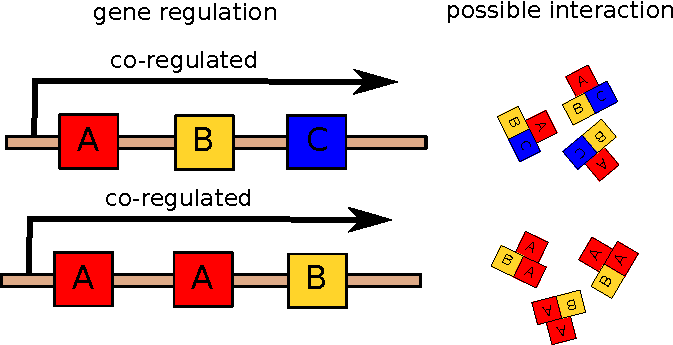
\includegraphics[width=0.5\linewidth]{Intro/Fig/CoRegulation.pdf}  
      \caption[Co-regulation scheme]{Example of a gene co-regulated cluster and the probable complex with the stechiometry set by the co-regulation.}
      \label{Fig:CoRegulation}
    \end{centering}
\end{figure}

\subsubsection{Phylogenetic profile methods}
These methods are based on the hypothesis that the interacting proteins coevolve and therefore have orthologous proteins among sequenced organisms \cite{barker2005predicting}.
If the proteins related to the two proteins in question are present in majority of organisms therefore, they probably constitute 
a pathway or physically interact. The phylogenetic profiles are constructed for the proteins where their presense indicated by 1 or 0. Then, these
profiles are clustered and the proteins belonging to one cluster are assumed functionally related or interacting.

\subsubsection{Rosetta Stone method}
This method relies on the observation that interacting proteins have homologs in other organisms that are fused into one protein. These types of proteins
are called Rosetta Stone proteins. This fusion is the limiting case of the co-expression optimization of functionally related proteins. Using this method
Marcotte \emph{et all} \cite{marcotte1999detecting} identified about 7,000 pair of potentially interacting proteins in \emph{E.Coli} and further analysis of the data revealed
that around a half of these pairs are functionally related.

\subsubsection{Co-evolution based methods}
During the evolution, mutations in one of the proteins of a complex should be compensated by the mutations in its partner in order to maintain the function (see Fig.\ref{Fig:CoEvolution}). 
The co-evolution based methods use the similarity measures between phylogenetic trees of two interacting protein families. Studies showed that some implementations 
of this method can predict up to 50\% of real interactions with false positive rate as low as 6.4\% \cite{pazos2001similarity}.

\begin{figure}[H]
    \begin{centering}
      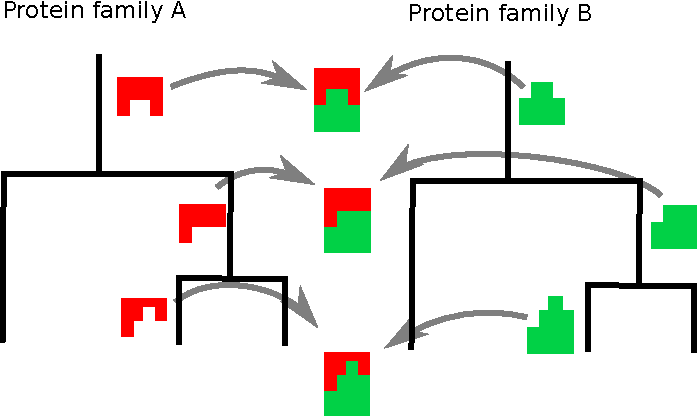
\includegraphics[width=0.5\linewidth]{Intro/Fig/CoEvolution.pdf}  
      \caption[Co-evolution scheme]{Example of a genes co-evolution where evolutionary changes in one protein compensate for the changes in its interaction partner.}
      \label{Fig:CoEvolution}
    \end{centering}
\end{figure}

\subsection{Bottom-up approaches}
Bottom-up approaches to the prediction of protein-prtoein interactions rely on the known structure of the proteins that constitute the complex.
The structures can either be modelled by homology, obtained using evolutionary constraints or taken from such experiments as NMR, X-Ray crystallography
or Cryo-EM. These methods are usually applied to infer the missing structural information about the protein-protein complex rather than to predict the fact
of interaction. 
Because bottom-up approaches use two or more protein structures that they dock into a complex, this class of techniques are usually called docking algorithms.
The pioneering work in this field was done by Janin and Wodak \cite{wodak1978computer}. Since then, this field has grown enormously, with its own
 quality assessment \cite{Mendez2003,Mendez2005,Janin2009}.
The two major parts of all the algorithms in this field are: sampling and scoring \cite{ritchie2008recent, huang2014search}. As the name suggest, the sampling part 
generates putative conformations of a complex of proteins and scoring ranks them according to some criteria. 

\subsubsection{Search strategies}
Suppose we have two molecules that are assumed to be rigid. One of the molecules (usually the one of a higher molecular weight) is called receptor and is fixed at the origin of the coordinate frame.
The other, called ligand, is moved around the receptor. The global search algorithm explores all possible rotations and translations of the ligand movements.
Complexity of this problem is $O(N^9)$, where $O(N^3)$ comes from rotational, $O(N^3)$ from the translational degrees of freedom and $O(N^3)$ is the complexity of the 
integration of the overlap integral that is computed for each rotation and translation of the ligand. A rough estimate
gives $\approx 10^{10}$\cite{huang2014search} operations. Several approaches allowed reducing this enormous complexity by at least an order of magitude.
These are the fast Fourier transform correlation and clever heuristics in the direct search.

\paragraph{FFT-based rigid body docking}
The idea to perform correlations in the Fourier space was first used by Katchalski-Katzir and colleagues \cite{katchalski1992molecular}. 
In this section I give a short description of this approach with a comprehesive 2D example.

Suppose that proteins receptor ($\mathbf{R}$) and ligand ($\mathbf{L}$) are represented as the numbers on a 3D grid:
\begin{eqnarray}
 R(l,m,n)= \begin{cases}
            1, (l,m,n)\in \mbox{surface of }\mathbf{R}\\
            \rho, (l,m,n)\in \mbox{inside of }\mathbf{R}\\
            0, (l,m,n)\in \mbox{outside of }\mathbf{R}
           \end{cases}
L(l,m,n)= \begin{cases}
            1, (l,m,n)\in \mbox{surface of }\mathbf{L}\\
            \delta, (l,m,n)\in \mbox{inside of }\mathbf{L}\\
            0, (l,m,n)\in \mbox{outside of }\mathbf{L}
           \end{cases}
           \label{Eq:LigRecGrid}
\end{eqnarray}
where $\rho\ll-1$ and $0<\delta<1$, according to the original work by Katchalski-Katzir \cite{katchalski1992molecular}. The shape complementarity score will therefore read:
\begin{equation}
 C(p,q,r)=\sum_{l,m,n=1}^{N} R(l,m,n)\times L(l+p,m+q,n+r),
\end{equation}
where the periodic boundary conditions are applied. Function $C$ defined on the same grid gives complementarity score that depends on the shift of the ligand $(p,q,r)$.
This function can be computed using the FFT algorithm as follows:
\begin{equation*}
 C(p,q,r)=\mbox{FFT}^{-1}\left[ \overline{\mbox{FFT}[\mathbf{R}]}\times \mbox{FFT}[\mathbf{L}]\right], \label{Eq:FFTDockingConvolution}
\end{equation*}
where $\mbox{FFT}^{-1}$ stands for the inverse fast Fourier transform and overline for the complex conjugate. This algorithm allows to rapidly sample translational degrees of freedom.
The rotations of the protein are separated from the translations in the outer loop of the algorithm. Fig. \ref{Fig:FFTDocking} shows a comprehensible example of 2D calculations
using this approach.

An example of the docking procedure is shown on Fig. \ref{Fig:FFTDocking}. The first row shows the picture of receptor and its Fourier image. The first column shows different
ligand poses. The border outlined with the dark-blue and the inner space with light-blue. The numbers placed on the grid are described by Eq. \ref{Eq:LigRecGrid}.
The second column shows the Fourier images of receptor and individual ligand poses. Third column shows the phases of Fourier image of the convolution 
$\mbox{FFT}[C(p,q,r)]=\overline{\mbox{FFT}[\mathbf{R}]}\times \mbox{FFT}[\mathbf{L}]$. The phases of the inverse Fourier transform of the data from the third column are
shown in the fourth one, it was computed according to Eq. \ref{Eq:FFTDockingConvolution}. Finally, in the last column the pose with the best score is shown, here the ligand is shown with the light-blue and the 
receptor is depicted with the dark-blue color. The images of Fourier transforms were built using the projection of complex values to the HSV colorspace \cite{PetrisonE2013visualizing} with the 
amplitude fixed to $V=100.0$.

\begin{figure}[H]
    \begin{centering}
      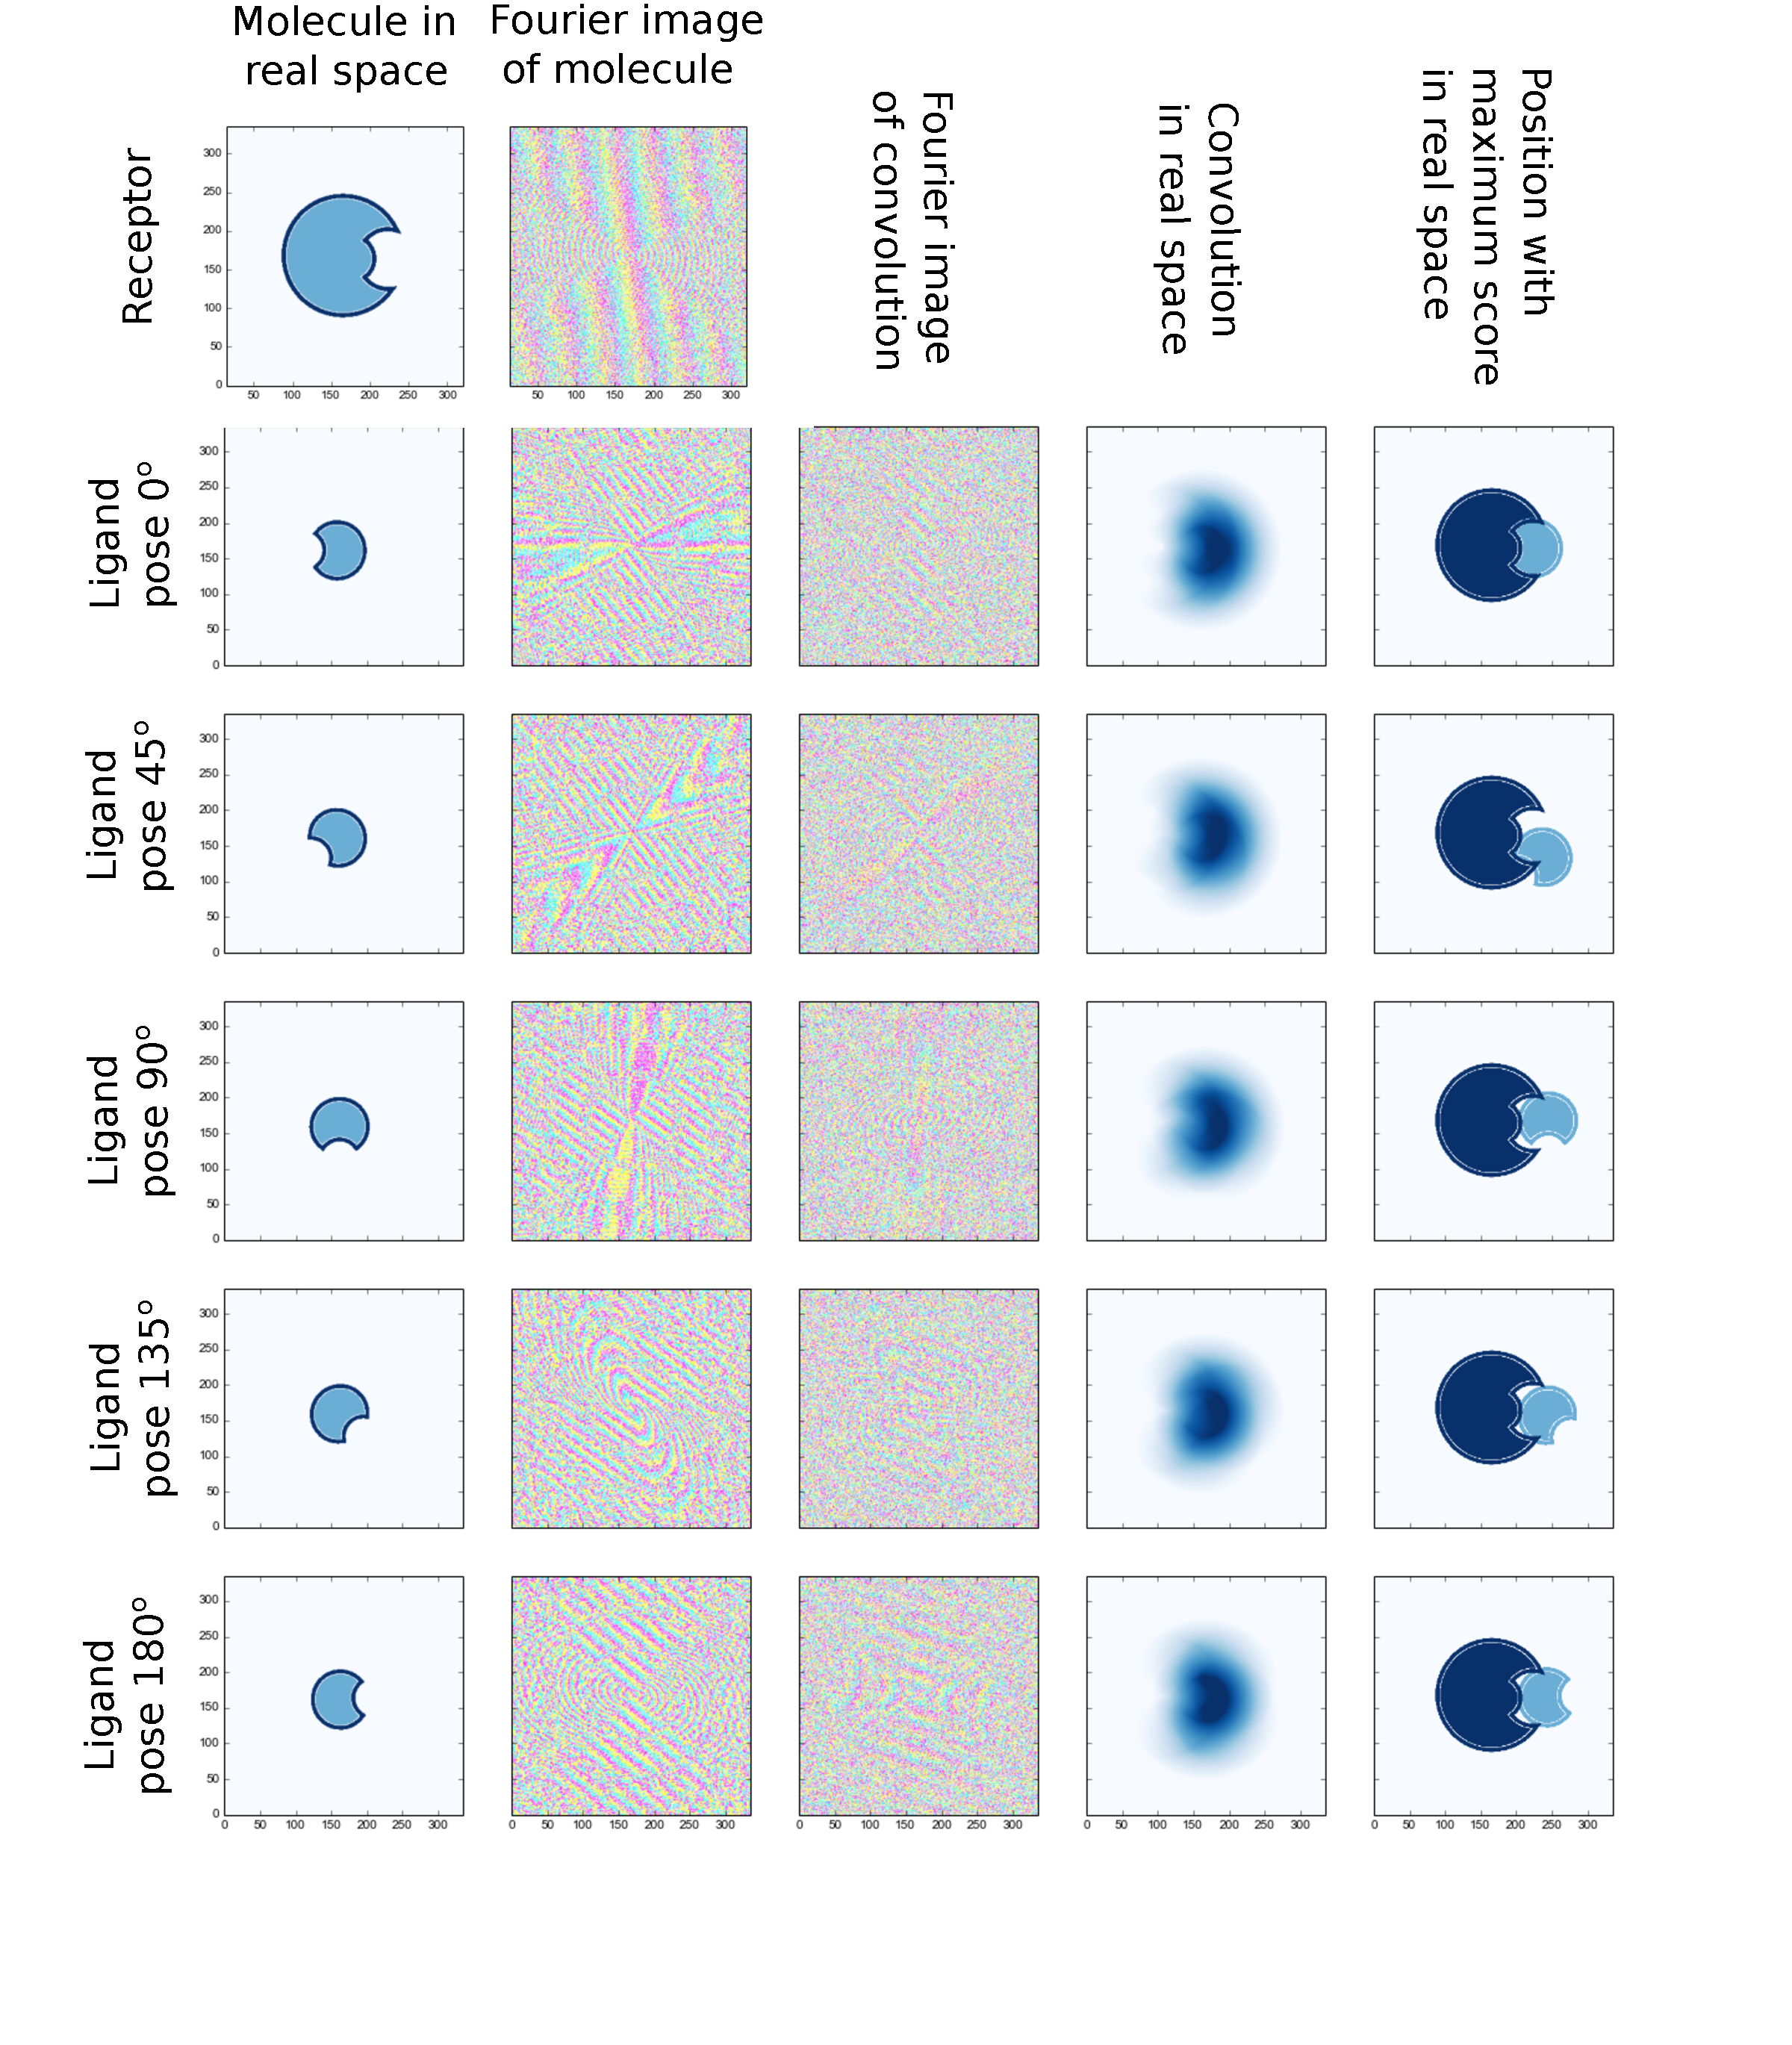
\includegraphics[width=1.0\linewidth]{Intro/Fig/DockingExample}  
      \caption[FFT-based docking example]{Example of a FFT-based docking procedure.}
      \label{Fig:FFTDocking}
    \end{centering}
\end{figure}


%In the modern algorithms based on the idea described above, a simple shape complementarity is usually coupled to the information about binding site  \cite{eben2003weighted}, 
%electrostatic energy \cite{gabb1997modelling}, atomic desolvation effect \cite{chen2002docking}, 
%knowledge-based potentials \cite{mintseris2007integrating}, \emph{etc}.

The algorithms that use FFT-based search strategies outnumber the algorithms relying on the other types of search strategies, 
to name a few: FTDock\cite{gabb1997modelling}, GRAMM\cite{vakser1997evaluation}, ZDOCK\cite{pierce2011accelerating}, PIPER\cite{kozakov2006piper}, \emph{etc}.
This technique is also used to accelerate the search not only in the space of translations but also in the rotational space \cite{garzon2009frodock,ritchie2000protein,ritchie2008recent} 
and even in 5D rotation-translational space .

\paragraph{Sophisticated scoring during exhaustive search}

In modern algorithms based on the idea described above, a simple shape complementarity is usually coupled to the information about binding site  \cite{ben2003weighted}, 
electrostatic energy \cite{gabb1997modelling}, atomic desolvation effect \cite{chen2002docking}, 
knowledge-based potentials \cite{mintseris2007integrating}, \emph{etc}.
The general idea behind the incorporation of additional scoring approaches can be shown on the example of the ZDOCK program \cite{mintseris2007integrating}.
The scoring function that is used in addition to shape complementarity in this algorithm contains the desolvation term, electrostatics and knowledge-based scoring
potentials.
To estimate the desolvation energy, the authors used atomic contact energies (ACE)\cite{chen2002docking}. It is defined as the free energy change of breaking two protein atom
contacts with water and forming a new contact between these two atoms. The pairwise shape complementarity (PSC) and ACE are represented on the grid 
in the following way:

\begin{eqnarray*}
 R_{PSC}=L_{PSC}=\begin{cases}
                  3 & \mbox{surface of a protein}\\
                  3^2 & \mbox{protein core}\\
                  0 & \mbox{empty space}
                 \end{cases}
\end{eqnarray*}

\begin{eqnarray*}
 \mbox{Re}\left[R_{DE}\right]=\mbox{Re}\left[L_{DE}\right]=\begin{cases}
                  \mbox{sum of ACE and PSC scores for nearby atoms} & \mbox{empty space}\\
                  0 & \mbox{otherwise}
                 \end{cases}
\end{eqnarray*}

\begin{eqnarray*}
 \mbox{Im}\left[R_{DE}\right]=\mbox{Im}\left[L_{DE}\right]=\begin{cases}
                  1 & \mbox{grid point is the nearest grid point of an atom}\\
                  0 & \mbox{otherwise}
                 \end{cases},
\end{eqnarray*}
where $R$ stands for receptor and $L$ - for the ligand. The final score is:
\begin{equation*}
 S_{PSC+DE}=\mbox{Re}\left[R_{PSC} \times L_{PSC}\right] + \frac{1}{2}\mbox{Im}\left[R_{DE} \times L_{DE}\right]
\end{equation*}
The electrostatic energy calculation is performed similarily:
\begin{eqnarray*}
 R_{PSC+ELEC}=L_{PSC+ELEC}=\begin{cases}
                  3 & \mbox{surface of a protein}\\
                  3^2 & \mbox{protein core}\\
                  0 & \mbox{empty space}
                 \end{cases}
\end{eqnarray*}
\begin{eqnarray*}
 \mbox{Im}\left[R_{PSC+ELEC}\right]=\begin{cases}
                  \beta \times \mbox{(electric potential of receptor)} & \mbox{empty space}\\
                  0 & \mbox{otherwise}
                 \end{cases}
\end{eqnarray*}

\begin{eqnarray*}
 \mbox{Im}\left[L_{PSC+ELEC}\right]=\begin{cases}
                  -1\times\mbox{(atom charge)} & \mbox{grid point is the nearest grid point of a ligand atom}\\
                  0 & \mbox{otherwise}
                 \end{cases}
\end{eqnarray*}
Finally, the total score is computed as follows:
\begin{equation*}
 S_{PSC+DE+ELEC}=\mbox{Re}\left[R_{PSC+ELEC} \times L_{PSC+ELEC}\right] + \frac{1}{2}\mbox{Im}\left[R_{DE} \times L_{DE}\right]
\end{equation*}
We see that using not only real part of the grid values but also their imaginary part, one can compute electrostatics, desolvation and 
shape complementarity using two convolution calculations.


\paragraph{Direct search in Cartesian space}
In this type of approaches the representation of the protein is also grid based, but simpler than in the FFT-based ones. 
Grid values are either 1 if the grid is occupied by the protein or 0 otherwise.
The algorithms from this category use boolean logic and heuristic rules to speed up the search \cite{jiang1991soft, terashi2007ske}.

\paragraph{Local shape matching}
Algorithms implemented in such programs as LZerD \cite{venkatraman2009protein}, GAPDOCK \cite{gardiner2001protein}, PatchDock \cite{duhovny2002efficient}, \emph{etc} 
represent protein as a set of surface patches. 
Efficient search algorithms match the surface patches on two proteins and recover the rotation and position of a candidate docking pose from the patches.

\paragraph{Randomized search strategies}
An example of this type of approaches is the package RosettaDock\cite{gray2003protein}. It generates random starting positions of a ligand around receptor. Afterwards,
it minimizes the score while moving the ligand along the line connecting their centers of masses. RosettaDock also uses different representations
of the protein at two distinct stages of minimization to reduce the number of degrees of freedom: coarse-grained and full-atom ones. The same methodology is used by the 
programs like ATTRACT \cite{zacharias2003protein}, HADDOCK \cite{dominguez2003haddock}, \emph{etc}. Another example of randomized search approach is the SwarmDock algorithm \cite{li2010detection}.
This program uses population-based search algorithm, called particle swarm optimization. Each copy of the protein-protein complex being optimized
is an agent. During optimization of each agent it shares information about its state with the neighbouring agents and they change the parameters of optimization accordingly. The 
particle swarm optimization algorithm is especially well suited for exploring energy landscapes with large number of local minima.

\subsubsection{Scoring candidate conformations}

Despite the vast variety of the methods to obtain the scoring functions, we can group
them into two major classes -- physics-based SFs and statistical
SFs. The first class of SFs is constructed as a weighted sum of terms,  such as desolvation \cite{Wang2003}, electrostatic interactions
\cite{Sheinerman2002}, hydrogen bonds \cite{Fernandez2003},
hydrophobic interactions \cite{Scarsi1999}, etc., given as  $E=\sum_{i}\alpha_{i}E_{i}$. Then,
the weights $\alpha_{i}$ are usually tuned to match some experiments
or to attain a minimum of the SF on a set of known structures of protein complexes. 
%
On the other hand,
statistical
SFs are developed based on the observation that the distances
between the atoms in experimentally determined structures follow the Boltzmann distribution \cite{finkelstein2004protein}.
%
More precisely, using ideas from statistical theory of liquids, effective potentials between
atoms are extracted using the inverse Boltzmann relation: $E_{ij}(r)=-k_{B}T\mbox{ln}\frac{P_{ij}(r)}{Z}$,
where $k_{B}$ is the Boltzmann constant, $P_{ij}(r)$ denotes the
probability to find two atoms of types $i$ and $j$ at a distance
$r$, and $Z$ denotes the probability distribution in the reference state. The latter is the thermodynamic equilibrium state of the protein when all
interactions between the atoms are set to zero. 
%
The score of a protein conformation is then given as a sum of effective potentials between
all pairs of atoms. Although this concept is old ( it originates from
the work of Tanaka and Scheraga \cite{Tanaka1976}, Miyazawa and Jernigan \cite{miyazawa1985estimation} and Sippl  \cite{sippl1990calculation} ),
it is still under
debates \cite{Thomas1996,Sippl1996,Sippl1997,ben1997statistical}. 
Particularly, the computation of the reference state is a challenging problem and only recently some
attempts to rigorously justify and compute it have been made \cite{Hamelryck2010}. Some scoring functions from this class were obtained without the computation of the 
reference state. Among those we should mention SF obtained using linear programming \cite{Tobi2000,Tobi2006,Vendruscolo2000},
quadratic programming, support vector machines \cite{Bernauer2007,Hu2004,Martin2008}, and iterative techniques \cite{Huang2008,Huang2010}.

Here I describe some examples of knowledge-based scoring functions, used in DFIRE \cite{zhou2002distance}, ATTRACT \cite{zacharias2003protein} and ZDOCK \cite{mintseris2007integrating} algorithms.
The approach chosen by the authors of DFIRE scoring function uses the ideal-gas reference state that allowed them to unify the folding and docking scoring functions.
The pair distribution function has the following dependence on the number of observed pairs:
\begin{equation*}
 N_{obs}(i,j,r)=\frac{1}{V}N_i N_j g_{ij}(r) 4\pi r^2 \delta r
\end{equation*}
Where $N_{obs}(i,j,r)$ is the number of observed atoms of $i$-th and $j$-th types at the distance $r$.
The potential of mean-force is connected to the pair distribution function: $u(i,j,r)=-RT \ln g_{ij}(r)$. When the interaction $u(i,j,r)$ is set to zero,
one obtains the distribution in the reference state $N_{exp}(i,j,r)=\frac{1}{V}N_i N_j 4\pi r^2 \delta r$.
However, due to the finite size of the protein, the correction coefficient $\alpha$ was introduced:
\begin{equation*}
 N_{exp}(i,j,r)=\frac{1}{V}N_i N_j 4\pi r^\alpha \delta r
\end{equation*}
The potential is assumed to have finite range and the equation for the potential is simplified by employing the pairwise distribution in the reference state at the potential cutoff distance:
\begin{equation*}
 N_{exp}(i,j,r_{cut})=N_{obs}(i,j,r_{cut})=\frac{1}{V}N_i N_j 4\pi r_{cut}^\alpha \delta r_{cut}
\end{equation*}
Finally, the form of the potential is the following:
\begin{eqnarray*}
 u(i,j,r)=\begin{cases}
                  -\nu R T \ln \frac{N_{obs}(i,j,r) }{\left(\frac{r}{r_{cut}} \right)^\alpha \left(\frac{\delta r}{\delta r_{cut}} \right) N_{obs}(i,j,r_{cut}) }, & r<r_{cut}\\
                  0 & otherwise
                 \end{cases}
\end{eqnarray*}
where $\nu = 0.0157$, R is the gas constant, T was set to 300K and $\alpha=1.61$. 
The $\delta r$ and $\delta r_{cut}$ are the widths of bins at the distances $r$ and $r_{cut}$ correspondingly. 
The coefficient $\nu$ was tuned to maximize correllation
between the experimental and the predicted stability upon the mutations of monomeric proteins. The exponential factor $\alpha$ is determined using the uniformly distributed
points in a sphere for each structure. The radii of the spheres were set to $cR_g$, where $R_g$ is the gyration radius of a protein and $c$ was tuned to equal the number of
pairs within the $r_{cut}$ for the reference state and the experimental structures.
Such a choice of the reference state implies that the information about the protein-protein contacts is negligible compared to the information on the interaction
withing proteins. This fact let the authors to unify folding and docking scoring functions.

D. Kozakov \emph{et. al.} developed the ``decoys as reference state'' (DARS) potential for scoring protein-protein interactions. The key idea was to dock the proteins in the training set 
using only shape complementarity term in the scoring of conformations. These structures simulate the absense of interactions between two proteins and were
used as the reference state. However due to computational complexity, the authors chose only 22 protein-protein complexes to derive the reference state.

Zacharias and his team used a different approach: they used only the Leenard-Jones type of interaction and the electrostatic interaction with distance-dependent dielectric constant $\epsilon=15r$.
They estimated the parameters of interaction potential using the similar approach as in the work by Miyazawa and Jernigan \cite{miyazawa1999self}.

\subsubsection{Knowledge-based potentials in rigid-body search}
During the rigid-body search algorithms typically filter out about $\approx 10^4$ conformations. Most of them are later refined by the scoring procedure. However, due to
a simple scoring function used during the search, the conformations that are close to the solution could be underrepresented in the output of rigid-body docking algorithms.
Therefore, two approaches exist to incorporate knowledge-based scoring functions into exhaustive 6D search procedure. 
One of them, used in the ZDOCK3.0 program \cite{mintseris2007integrating} integrates atomic contact potential into 6D search procedure in the following way. Suppose
one has 2N atom types. For the ligand, N functions on a grid are defined in the following way:

\begin{eqnarray*}
 \mbox{Re}\left[L_{i}\right]=\begin{cases}
                  1 & \mbox{if grid cell is occupied by a ligand atom type i}\\
                  0 & \mbox{otherwise}
                 \end{cases}\\
 \mbox{Im}\left[L_{i}\right]=\begin{cases}
                  1 & \mbox{if grid cell is occupied by a ligand atom type i+1}\\
                  0 & \mbox{otherwise}
                 \end{cases}
\end{eqnarray*}
The N functions for the receptor are:
\begin{eqnarray*}
 \mbox{Im}\left[R_{i}\right]=\begin{cases}
                  \sum e_{i,j} & \mbox{Neighbours within }r_{cut}\\
                  0 & \mbox{non-neighbour atoms}
                 \end{cases}\\
 \mbox{Re}\left[R_{i}\right]=\begin{cases}
                  \sum e_{(i+1),j} & \mbox{Neighbours within }r_{cut}\\
                  0 & \mbox{non-neighbour atoms}
                 \end{cases},
\end{eqnarray*}
where $e_{i,j}$ is the value of the contact potential between atom types $i$ and $j$ and $r_{cut}$ is the contact radius. The sum of contacts looks as follows:
\begin{equation*}
 E = \sum^{2N}_{i=1}\sum^{2N}_{j=1}e_{ij}n_{ij} = \sum^{N}_{k=1}\left[\sum_{x,y,z} L_i \times R_i \right]
\end{equation*}
Thus, to compute the contact potential energy one has to perform $N$ forward Fourier transforms and one backward (due to additivity of energy).

Despite the usage of both complex and real parts during the computation of contact potentials $N$ can be around 10, which slows drastically the rigid-body docking algorithm.
In order to reduce the number of Fourier transforms Kozakov \emph{et. al.} \cite{kozakov2006piper} proposed to decompose the interaction matrix $e_{i,j}$ into the eigenvectors:
\begin{equation*}
 e_{i,j} = \sum_p^P \lambda_p u_{p,i} u_{p,j}
\end{equation*}
where $P$ depends on the allowed error rate. Ususally the aproximation of the pairwise potential energy using the grid yelds 10\% error in energy, therefore the truncation
of the decomposition is well justified. The functions for the receptor and the ligand look like:

\begin{eqnarray*}
 R_{p}=\begin{cases}
                  \sum_i u_{p,i} & \mbox{Over all neighbours $i$ within }r_{cut}\\
                  0 & \mbox{no neighbour atoms}
                 \end{cases}\\
 L_{p}=\begin{cases}
                  u_{p,j} & \mbox{If atom of type j is in the cell}\\
                  0 & \mbox{otherwise}
                 \end{cases}
\end{eqnarray*}
This approach allows to compute only four Fourier correlations with the same error as in the previous algorithm.

\subsubsection{Modelling of water molecules}

An important part of a protein-protein interface constitute the water-mediated interactions. One pronounced example of the protein-protein complex where 
water molecules play great role is the barnase-barstar complex. In the interface of this complex 18 water molecules are fully burried mediating a considerable 
amount of sidechain-sidechain interactions \cite{buckle1994protein}. Water molecules also play a role in the interaction 
between protein and drug-like molecules \cite{ben2002molecular,huggins2011systematic}. 

In spite of the importance of the water molecules prediction for the drug desing, numerous works are devoted to predict positions of water molecules 
around a known protein structure \cite{forli2012force, wang2011ligand, ross2012rapid}. However, the amount of papers attempting to predict the explicit solvation of protein-protein 
interfaces is substantially less \cite{jiang2005solvated,bui2007watgen,kastritis2013solvated,ahmad2011adhesive}.

Historically, the first approach to account for the water-mediated interactions during protein-protein docking was the use of the \emph{solvated rotamers} \cite{jiang2005solvated}. The key idea
of this method is to attach the water molecules to the functional groups of the residues and the backbone and treat different solvation modes as rotamers. Fig \ref{Fig:SolvatedRotamer} shows
an examples of water molecules placement around aromatic nitrogen in histidine.

\begin{figure}[H]
    \begin{centering}
      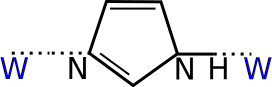
\includegraphics[width=0.4\linewidth]{Intro/Fig/SolvatedRotamer}  
      \caption{Water molecules placement around aromatic nitrogen in histidine residue functional group.}
      \label{Fig:SolvatedRotamer}
    \end{centering}
\end{figure}
The water molecules placement around the protein was derived by the authors from X-Ray crystallographic structures solved at high resolution. To avoid combinatoric explosion of
the number of solvated rotamers they restricted the placement of water molecules to the non-adjacent sites in a protein.

The other approach was implemented in the algorithm WATGEN \cite{bui2007watgen}. First, the hydrogens are added to the interacting proteins. These hydrogens, that interact with 
the atoms of a protein are called donors. Afterwards, all possible positions of water molecules are generated and those which have clashes with the atoms of the two proteins are
discarded. Then, the water sites are selected based on the number of interactions they are involved into. Additionally, two water sites closer than 0.5\AA~ are considered equal.
Finally, geometry of the water hydrogens is optimized to maximize the number of interactions.



\subsubsection{Multimeric docking}
Methods and algorithms described previously are applicable mainly to the problem of doking dimeric protein-protein complexes. However, 
many proteins in a cell form multimeric assemblies that play crucial role in recycling of the proteins in a cell, folding of the proteins, translation, transcription and many other 
vital cellular processes. There are two major ways in deciphering the structure of a multimeric complex starting from its subunits. The first type of programs
do not rely on any other information except for the possible symmetry of a complex and the structures of its subunits. The second one uses low-resolution
electron density maps, obtained from cryo-EM or small angle neutron scattering experiments.

The first class of methods deals with complexes of two general types: symmetric and nonsymmetrical.
The number of packages that can do symmetry-based multimeric docking is quite small: SymmDock \cite{schneidman2005geometry}, 
can build complexes with cyclic symmetry; Rosetta program protocol, that uses Monte-Carlo approach and can take into account cyclic, dihedral, helical and
icosahedral symmetries \cite{andre2007prediction}; M-ZDOCK \cite{pierce2005m} reduces rotational search space assuming cyclic symmetry and relies on FFT-based docking approach, \emph{etc}.

A few programs can dock proteins into nonsymmetrical complexes: CombDock \cite{inbar2005prediction} uses combinatorial approach, generating all pairwise 
pairs and finding among them tripples with the optimal score; Kim and Hummer algorithm \cite{kim2008coarse}, which uses Monte-Carlo approach and coarse-graining the protein models, 
HADDOCK \cite{dominguez2003haddock}; ATTRACT \cite{zacharias2003protein}; Multi-LZerD \cite{esquivel2012multi} and DockTrina \cite{popov2014docktrina}.

However, despite the variety of methods, they still perform poorly even on a simple benchmark \cite{popov2014docktrina}. The most reliable and widely-used technique 
to obtain atomic structure of a multimeric assembly is the docking of subunits into a low-resolution electron density map, usually obtained from cryo-EM experiments.

\paragraph{Docking proteins into low-resolution electron density map}
For this task, a number of software packages have been developed. 
Most notable of them are Situs \cite{Wriggers2010,Chacon2002}, NORMA \cite{Suhre2006},
EMFit \cite{Rossmann2001}, UROX \cite{Siebert2009}, etc. Despite the
differences in the implementation, all algorithms maximize
some score that shows the goodness of the fitting using a certain
optimization algorithm. An excellent review on different types of
the scoring functions used for cryo-EM density fitting is given by
Vasishtan and Topf \cite{Vasishtan2011}. According to them, one of
the most popular scoring functions is the cross-correlation function
(CCF) between the EDM and the density of the fitted protein. 

Given a protein structure that is described by its electron density $f(\mathbf{r})$,
and an EDM obtained from e.g. a cryo-EM experiment described by the function
$g(\mathbf{r})$, we can minimize the square root discrepancy between
them. Precisely, this discrepancy is given by
\begin{equation}
S=\int d\mathbf{r}\,\left(\hat T \hat R f(\mathbf{r})-g(\mathbf{r})\right)^{2},
\end{equation}
where $\hat T$ and $\hat R$ are the operators of the translation and the rotation
respectively, applied to the density $f(\mathbf{r})$. We can rewrite
the scoring function $S$ as 
\begin{equation}
S=\int d\mathbf{r}\,\left(\hat T \hat R f (\mathbf{r})\right)^{2}+\int d\mathbf{r}\, g^{2}(\mathbf{r})-2\int d\mathbf{r}\, \hat T \hat R f(\mathbf{r})g(\mathbf{r})
\end{equation}
Therefore, the minimization of the score $S$ is equivalent to the maximization
of the CCF: 
\begin{equation}
\textrm {CCF}=\int d\mathbf{r}\, \hat T \hat R f(\mathbf{r})g(\mathbf{r})
\end{equation}
with respect to the parameters of the operators $\hat T$ and $\hat R$. This
scoring function has been used in the majority of the algorithms and software
packages that perform the fitting into the EDM \cite{Wriggers2010,Siebert2009,Suhre2006}.

Another widely used scoring function is the Laplacian-filtered cross-correlation
function (LCCF). It originated from the observation that a human
performing a manual fitting a structure into an EDM tends to match
the isosurfaces of the densities rather than the densities themselves,
\begin{equation}
\textrm {LCCF}=\int d\mathbf{r}\,\left(\triangle \hat T \hat R f(\mathbf{r})\right)\left(\triangle g(\mathbf{r})\right)
\end{equation}
This scoring function works better than CCF for low resolution maps ($\sim 10-30$~\AA) \cite{Wriggers2010} and was used for the first time in the CoAn/CoFi
algorithm \cite{Volkmann1999}. Other scoring functions
that e.g. penalise symmetry-induced protein-protein contacts, or make use of protein-protein docking potentials, etc., have also been developed \cite{Vasishtan2011}.
